\section{Custom Python Scripts (SymPy)}
    \begin{frame}
        \frametitle{Optimization: Difference of V(t) for Hopping}

        \begin{columns}
            \column{0.4\textwidth}
                \begin{itemize}
                    \onslide
                    \item Monte-Carlo sampling requires transition probabilities between "adjacent" states
                    \pause
                    \item These require differences of $\hat{V}^\mathrm{I}(t)$ and $E_0$
                    \pause
                    \item Too many terms for simple evaluation by hand
                    \item Intelligent pre-computation required to speed up processing
                \end{itemize}
            \column{0.4\textwidth}
                \onslide
                \makebox[\textwidth][c]{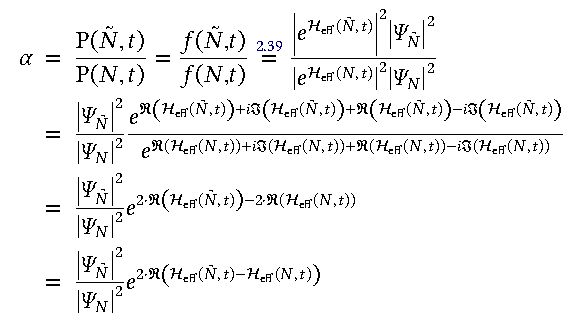
\includegraphics[width=1.3\textwidth]{main-content/python/sampling-probability.pdf}}
                
        \end{columns}

        % notes 
        \onslide % on all slides of frame
        \note[item] {
            "Adjacent" states because from one Monte-Carlo step to the next we require a small change of one or two particle-sites. Could come from hopping or flipping.
        }
        \note[item] {
            The $E_0$ differences are quickly calculated by hand in the report
        }
    \end{frame}

    \begin{frame}
        \frametitle{The process: Difference of V(t) for Hopping}
        
        \hspace{-1cm}
        \makebox[\textwidth][c]{
            \onslide<1->
            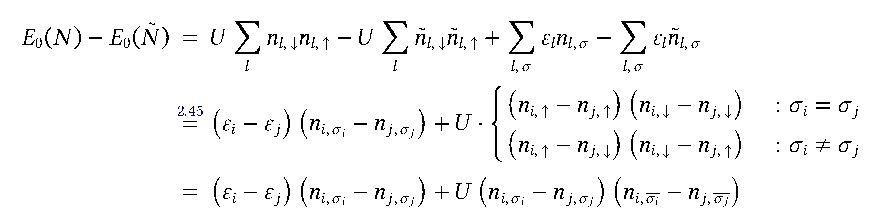
\includegraphics[width=0.7\textwidth]{main-content/python/hopping-e0-example.pdf}
            \onslide<2->
            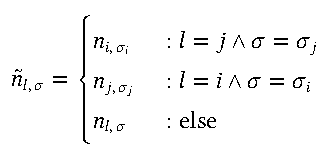
\includegraphics[width=0.28\textwidth]{main-content/python/n-redefinition.pdf}
        }

        \vspace{0.3cm}

        \begin{itemize}
            \onslide<1->
            \item Setup difference
            \onslide<2->
            \item Replace one by appropriate new occupation
            \onslide<3->
            \item Simplify as much as possible
            \item Sum over all possible neighbor combinations
        \end{itemize}

        \vspace{0.1cm}
        
        \onslide<4->
        \textbf{Problem:} number of terms/combinations: $3 \cdot 8 \cdot 4 \cdot 2 = 192$

        % notes 
        \onslide % on all slides of frame
        \note[item] {
            The $V$ differences are $3 \cdot 8 \cdot = 32 \cdot 4 = 96 \cdot 2 = 192$ terms
        }
        \note[item] {
            The process is relatively straight forward:
            \begin{itemize}
                \item write down the terms
                \item replace
                \item simplify difference
            \end{itemize}
        }
        \note[item] {
            Still quite complicated and a lot of work, but: 
            \begin{itemize}
                \item way faster to write bacuse non-repetetive logic
                \item verifiably correct calculations
                \item multiple times re-done on changes to underlying code, each time only took seconds
                \item sometimes brute-force NEEDS to work, before optimization can be found
            \end{itemize}
        }
    \end{frame}

    \begin{frame}
        \frametitle{Script-Generation: Difference of V(t) for Hopping}
        
        \begin{block}{Generating Script}
            \href{https://github.com/jonas-kell/master-thesis-code/blob/master/calculation-helpers/simplificationtermhelper.py}{simplificationtermhelper.py}
        \end{block}

        \vspace{1cm}

        \begin{block}{Generated Script}
            \href{https://github.com/jonas-kell/master-thesis-code/blob/master/computation-scripts/analyticalcalcfunctions.py}{analyticalcalcfunctions.py}
        \end{block}

        % notes 
        \onslide % on all slides of frame
        \note[item] {
            \texttt{simplificationtermhelper.py} script to generate the script
        }
        \note[item] {
            \texttt{analyticalcalcfunctions.py} script is generated and used in the code
        }
        \note[item] {
            Generated file: 1556 lines, script that generates: 534 lines
        }
        \note[item] {
            Show the script that generates/is generated $\rightarrow$ simplification with Sympy \item Parallel to computer-science practice "Vendored" code
        }
    \end{frame}